%!TEX root = ../thesis.tex
\chapter{Keyword Spotting with efficient convolutions} \label{ch:kws}

\section{Overview}
Speech commands recognition is a very important task nowadays due to the increase of the global interest in personal assistants. The field of conversational agents is growing fast and there is an increasing need for algorithms that perform well in order to enhance natural interaction. In this work we show how we achieved state of the art results by adapting and tweaking the \textit{Xception} algorithm, published by François Chollet in 2017, which achieved outstanding results in several computer vision tasks. This architecture is designed to exploit the computational benefits and efficiency of the \textit{depthwise-separable convolutions}, leading to a solution with significantly lower computational requirements than a regular convolutional neural network. We obtained about 96\% accuracy when classifying audio clips belonging to 35 different categories, beating human performance at the most complex benchmarks proposed.

This study has been published in the proceedings of the \textit{European Symposium of Artificial Neural Networks} (ESANN 2021) \cite{valles2021a}. The content of this chapter is almost identical to the content of the manuscript, with minor modifications and adaptions. All the code used to generate the results presented in this chapter is included in a public repository \footnote{\url{https://github.com/ivallesp/Xception1d}}.

\section{Introduction}
The world of voice-activated virtual assistants is booming. Several giant technological companies, (such as Amazon, Google, Apple and Baidu) have already developed their version of a virtual assistant. There is a huge research community surrounding this field, potentially promoted by the recent growth of the artificial intelligence (AI) paradigm.

There has been an outstanding evolution in this field, leveraging AI and machine learning (ML) advances for  making virtual assistants behave as close as humans as possible. There are multiple open research lines, such as increasing the accuracy and the relevance of the responses \cite{milabot2017}, reducing the answer delay \cite{Han2017} or increasing their variability of the responses \cite{Li2017}. In particular, Deep Learning (DL) models have revolutionized the field of automatic speech recognition \cite{Nassif2019}, as language features are highly hierarchical. This work focuses on DL models to increase the accuracy of a voice command recognition task using a limited vocabulary.

An important factor to take into account is the small size and low power specifications of the usual virtual assistants, which limit the complexity of the models to implement. Furthermore, a low latency is needed to avoid harming the users' experience. DL models usually contain millions of parameters. For that reason, the right choice of number of layers and their architecture is critical. Using the cloud for processing audio commands can partially mitigate this. However, continually transmitting to and from the cloud increases latency and may not be an efficient solution. Therefore, at least the models that process the most common words in a vocabulary, such as keyword spotting (KWS), should be implemented locally.

The current commercial virtual assistants are still not as accurate as humans at identifying human voice commands \cite{Michaely2017}. Although substantial efforts have been made and nearly human performance has been reported in several studies \cite{Andrade2018, Zhang2017, McMahan2018, Warden2018}, there is still room for improvement. In particular, bidirectional recurrent models with attention have been used  \cite{Andrade2018} as these kind of structures are able to accurately model past and future dependencies in the time domain, while attention focuses on important parts of the audio clip. Howewer, the authors state that there are word pairs that are difficult to identify without extra context. Gated convolutional long-short term memory (LSTM) structures have also proven useful by other authors \cite{Wang2018} to improve the state of the art results on the same data. According to this work, gated convolutions help further learn the local features of speech, improving the model prediction accuracy.

Due to their architecture, convolutional neural networks (CNNs) provide a good approach to optimize computational resources for KWS. In \cite{Tara2015}, CNNs outperform other deep neural networks (DNNs) architectures, such as recurrent reural networks (RNN), for the constrained KWS task. Other works focus on the hardware implementation of neural networks for KWS \cite{Zhang2017}, comparing not only their accuracy, but also their memory usage and computation efficiency. According to this work, Deepwise Separable (DS) CNNs achieve both the best accuracy and scalability among the tested architectures.  Transfer learning has also been applied to CNN architectures \cite{McMahan2018}, showing substantial improvements in accuracy.

The present work provides the insights of the study and implementation of an \textit{Xception}\footnote{\textit{Xception} is a deep CNN architecture that involves Depthwise Separable Convolutions.} based architecture \cite{FChollet2017}, which we named \textit{Xception-1d}, to the speech commands recognition problem.  The contributions of the present work are summarized in the following bullets.

 \begin{itemize}
 	\item Design and implementation of a \textit{depthwise separable} CNN-based architecture able to surpass the current state of the art results and the human performance while keeping the data in the temporal domain (using the raw version of the waveform).

 	\item Development of a new methodology (to the best of our knowledge) for augmenting audio data to increase the size of a data set (5x in this work), and therefore enhance generalization.

 	\item Quantification of the human performance across the different classification tasks to use it as an additional baseline for checking the results achieved by the algorithm.

	\item Creating a public repository where further contributions could be handled to enhance the project functionalities and to facilitate reproducibility.
 \end{itemize}

 The article is structured as follows. Right after this introduction, section \ref{sec:MM} introduces the data that has been used to define the tasks to be solved and the methodology and algorithms that have been used in order to achieve the results presented in section \ref{sec:results}. Section \ref{sec:discussion} provides a discussion of the results and section \ref{sec:conclusion} summarizes the insights, takeaways and possible future work lines.

 \section{Material and methods} \label{sec:MM}

\subsection{Data set}
One of the major contributions to the collection of open data sets in the field of speech commands recognition has been made by \textit{Google} with the release of the \textit{Google Tensorflow speech commands data set} \cite{speechcommands, Warden2018}. It consists of a collection of thousands of utterances with a length of one second containing short words, recorded by thousands of people. The recordings were collected remotely, in uncontrolled environments (i.e. without any specific quality requirements). The subjects were asked to say a chain of words during a minute. Then, the recordings were split in clips of one second by extracting the loudest sections of the signal \cite{speechcommands, Warden2018}.

Two different versions of the \textit{Google Tensorflow speech commands data set} have been used for quantifying the performance of the algorithm across the different tasks, described subsequently. The versions 0.01 and 0.02 of the data set contain 64,721 and 105,829 audio clips of one second (each one containing the recording of one voice command), respectively, with a sample rate of 16 kHz and 16-bit resolution. Each of them is stored in \textit{wav} format. The first data version has up to 30 different commands while the second one has 35 of them. The frequency distribution of the labels is described in Figure \ref{fig:freqdistdata}. For simplicity, we will refer to versions 0.01 and 0.02 as V1 and V2, respectively, from now on.


\begin{figure}[ht]
	\centering
	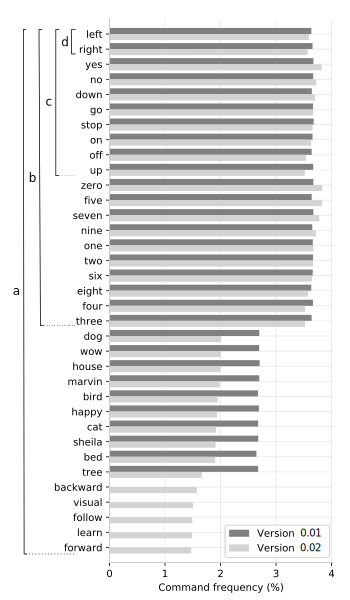
\includegraphics[width=0.45\linewidth]{kws/images/freqdist_data}
	\caption{Command frequency distribution for both versions of the data set. The V2 is a refined and extended version of V1. In the left, the four different tasks that have been benchmarked in this work: (a) referred as \textit{35-words-recognition} and comprising in both cases all the words for classification, (b) referred as \textit{20-commands-recognition}  (c) referred as \textit{10-commands-recognition} (d) referred as \textit{left-right} recognition.}
	\label{fig:freqdistdata}
\end{figure}

Four different tasks have been defined in order to benchmark the proposed algorithm. They are thoroughly described below in decreasing complexity order.

\begin{itemize}
	\item \textit{35-words-recognition}: consists of classifying all the different existing clips (commands and plain words) in each of the different categories (
	``left'',
	``right'',
	``yes'',
	``no'',
	``down'',
	``up'',
	``go'',
	``stop'',
	``on'',
	``off'',
	``zero'',
	``one'',
	``two'',
	``three'',
	``four'',
	``five'',
	``six'',
	``seven'',
	``eight'',
	``nine'',
	``dog'',
	``cat'',
	``wow'',
	``house'',
	``bird'',
	``happy'',
	``sheila'',
	``marvin'',
	``bed'',
	``tree'',
	``visual'',
	``follow'',
	``learn'',
	``forward'',
	``backward''). In the version V1 of the data set there are 5 missing commands and hence, the task consists of a 30-class classification task even though it is called \textit{35-words-recognition}.
	\item \textit{20-commands-recognition}: entails the categorization of all the clips representing the most commonly used commands in robotics \cite{Warden2018} and numbers (``left'',
	``right'',
	``yes'',
	``no'',
	``down'',
	``up'',
	``go'',
	``stop'',
	``on'',
	``off'',
	``zero'',
	``one'',
	``two'',
	``three'',
	``four'',
	``five'',
	``six'',
	``seven'',
	``eight'',
	``nine''), while the remaining words are grouped together in a synthetic category named ``unknown''.
	\item \textit{10-commands-recognition}: requires categorizing all the clips representing the typical commands in robotics (``left'',
	``right'',
	``yes'',
	``no'',
	``down'',
	``up'',
	``go'',
	``stop'',
	``on'',
	``off''), while the remaining clips are grouped together in a synthetic category named ``unknown''.
	\item \textit{left-right-recognition}: consists of categorizing the clips belonging to the ``left'' and ``right'' categories, while the rest of clips are grouped under the ``unknown'' category.
\end{itemize}


While it is true that, as we group the unrecognized words under the ``unknown'' category, the imbalance grows, in this kind of systems (speech recognition agents), the precision should be optimized at the expense of a worse recall (in general, the cost of a false positive is higher than that of a false negative). Thus, for our purpose, having a positive imbalance towards the ``unknown'' class does not represent an inconvenience. A summary of the percentage of words grouped under the ``unknown'' category for each task is shown in Table \ref{tab:unknowns}.

\begin{table}[ht]
	\centering
	\caption{Percentage of words represented by the ``unknown'' category in each one of the proposed speech recognition tasks. }
	\label{tab:unknowns}
	\begin{tabular}{lcccc}
		\hline
		Data set version & \textit{35-words} & \textit{20-commands} & \textit{10-commands} & \textit{left-right}  \\
		\hline
		V1 	& 0.00$\%$  &  26.84$\%$  &	  63.41$\%$  &	92.71$\%$ \\
		V2 	& 0.00$\%$  &	26.81$\%$  &  63.58$\%$  &	92.84$\%$ \\
		\bottomrule
	\end{tabular}
\end{table}


\subsection{Data augmentation}
Five different augmentations\footnote{meaning distorted versions of each of the clips in the original data} consisting of the application of a set of distortions have been performed to each and every audio clip. These distortions consist of a set of transformations being applied together over all the clips randomizing their parameters and intensities in each case. The different distortions used in this step are described below.

\begin{itemize}
	\item \textbf{Resampling}: the audio clip is resampled extending or contracting its length and hence changing its pitch \cite{Proakis2007}. If the resampling factor is lower than one, the audio clip is contracted and then the audio duration is zero-padded to keep the original duration of the original clips. On the contrary, if the resampling factor is greater than one, the audio clip is extended and a \textit{center-crop} operation is performed in order to keep the original length of one second.
	\item \textbf{Saturation}: the amplitude of the clip is increased by a given factor, potentially saturating the audio clip. The higher the factor, the larger the saturation of the clip \cite{Proakis2007}.
	\item \textbf{Time offset}: the audio clip is displaced in time by appending a set of zeros to the beginning of the signal and cropping the end (right offset) or by cropping a set of samples from the beginning, and adding the same number of zeros at the end (left offset) \cite{Proakis2007}.
	\item \textbf{White noise addition}: white noise (with gaussian distribution) is added to the clips with a given amplitude \cite{Proakis2007}.
	\item \textbf{Pitch shift}: the pitch of the clips is increased or decreased a given amount, producing higher or lower-pitched sounds \cite{Proakis2007, Szymon2016}.
\end{itemize}

All the distortions are applied together with random intensities only to the training data, producing 5 new transformations of the original recordings with high variability of results. These new versions are appended to the original data set.


\subsection{Methods}
We propose the use of a CNN with \textit{depthwise separable convolution} layers and \textit{residual connections}, based on the \textit{Xception architecture}  described by \textit{François Chollet} in 2017 \cite{FChollet2017}. This model is a CNN-based architecture which recently achieved state of the art results in multiple computer vision tasks \cite{Liu2019, Nazar2018, Song2018, Arriaga2017}.

\subsubsection{Depthwise separable convolutions}
The \textit{regular convolution} operation consists of the application of a filter over a signal along the spatial/temporal dimension(s) and along the channels in a single operation.

A \textit{depthwise separable convolution} performs an operation which, given an input tensor, produces an output tensor of the same shape that the regular convolution would produce, but in a more efficient way; i.e. it reduces the number of sums and multiplications needed to produce the output \cite{FChollet2017}. This is achieved by following the two steps described below. The whole operation is shown in the Figure \ref{fig:dwsconv}.



\begin{enumerate}
	\item \textit{Depthwise convolution} \cite{Yunhui2019}: consists of convolving a separate filter per channel. It produces an output tensor with potentially a different spatial/temporal dimensions size than the input (depending on the stride, the size and the padding of the convolution operation to be applied). However, the number of channels of the output tensor is constrained to be the same as the input.
	\item \textit{Pointwise convolution} \cite{Gao2018}: consists of applying a set of size-1 convolutions (as many as number of output channels desired). This operation can modify the channels dimension, leaving the spatial/temporal dimensions intact.
\end{enumerate}

Please refer to the appendix 1 to see the proper mathematical definitions.

\begin{figure}[ht]
	\centering
	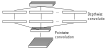
\includegraphics[width=0.65\linewidth]{kws/images/dws_conv}
	\caption{\textit{Depthwise separable convolution} diagram showing how the whole computation is done in two steps: the \textit{depthwise convolution} followed by the \textit{pointwise convolution}.}
	\label{fig:dwsconv}
\end{figure}



The \textit{depthwise convolution} does not combine different channels for producing the output, and hence always produces an output tensor which has the same number of channels as the input tensor. This difference makes this operation much more efficient than the \textit{regular convolution}, at the cost of loosing the ability to generate new features by combining different channels. That is the reason why the \textit{pointwise convolution} is applied after the \textit{depthwise convolution} constituting the \textit{depthwise separable convolution}. The reason why the \textit{separable} term is used in the name of the operation is because we are effectively separating between the channel-wise and the spatial/temporal-wise computations. The number of sums and multiplications required by this operation is $\frac{1}{N} \cdot \frac{1}{S}$ times the number of operations required by a regular convolution \cite{howard2017}, where $S$ is the size of the \textit{depthwise convolution} filters and $N$ is the number of output channels after the \textit{pointwise convolution} is applied. This represents a meaningful performance improvement for big networks.



\subsubsection{\textit{Xception-1d} architecture}
The proposed architecture exploits the gain in efficiency of the \textit{depthwise separable convolution} operation over the \textit{regular convolution} in the same way original \textit{Xception} does \cite{FChollet2017}. That allows a more efficient resource and time management and hence, a more complex architecture can be defined.

The \textit{Xception-1d} architecture is shown in Figure \ref{fig:arch}. It has a total of 37 layers, 34 of which are \textit{depthwise separable convolutional layers}, 2 of them are \textit{regular convolutions}, and the last one is a dense layer performing a logistic regression. The network contains 12 residual connections, one in each residual block, as shown in Figure \ref{fig:xceptionmodule}. All of it builds up a network with up to 21 million parameters in the case of the \textit{left-right recognition}  task and 23 million parameters in the \textit{35-words recognition} one\footnote{The difference lays on the last layer implementing the logistic regression of the architecture. Depending on the number of outputs required by each task, the number of parameters in this layer varies. The maximum difference occurs between the \textit{35-words recognition} task and the \textit{left-right recognition}}.

\begin{figure}[ht]
	\centering
	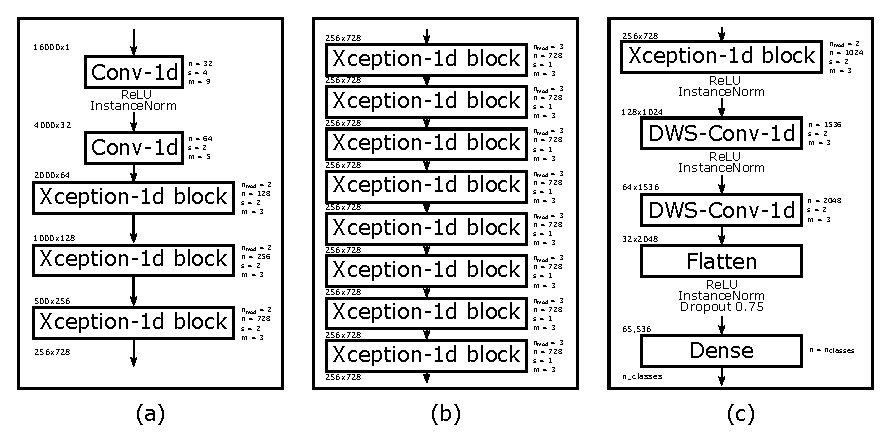
\includegraphics[width=1.0\linewidth]{kws/images/arch.eps}
	\caption{Diagram of the architecture used in this work where $n$ refers to the number of channels, $s$ is the stride of the convolutions (which in the case of the \textit{Xception-1d blocks} is applied through the final pooling operation), $m$ is the size of the convolution filters, $n_{mod}$ is the number of the \textit{depthwise convolutional} layers stacked in the \textit{Xception-1d blocks} (see Figure \ref{fig:xceptionmodule}) and $n_{classes}$ is the number of outputs of the network (i.e. the number of classes to predict, which depends on the task being solved). The architecture is built up in 3 main modules: (a) the entry module is the part of the network responsible for adapting the input wave into a condensed representation (by applying strides after each operation), (b) the middle module is responsible for learning the representation extracting the useful features that will allow the next module to distinguish between classes and (c) the classification module is responsible for mapping the extracted features into the number of outputs required for every task.}
	\label{fig:arch}
\end{figure}


\begin{figure}[ht]
	\centering
	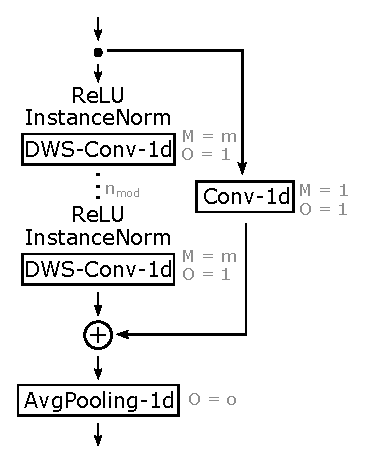
\includegraphics[width=0.4\linewidth]{kws/images/xception_module.eps}
	\caption{Neural network module refered as \textit{Xception-1d block}. The \textit{Xception-1d block} represents the building block of the architecture proposed in this work. It consists of a set of $n_{mod}$ \textit{1-D depthwise separable convolution} layers with a \textit{residual connection} and with a \textit{1-D average pooling} layer at the end. The activation function used is the \textit{rectified linear unit} (ReLU) and the normalization procedure after each convolutional layer is the \textit{instance normalization} for one dimensional sequences.}
	\label{fig:xceptionmodule}
\end{figure}



Considering that the last dense layer can be prone to overfitting due to the high number of parameters ($\sim 65,000$), a strong dropout \cite{srivastava2014, Goodfellow2016} has been applied after the last convolution ($p = 75\%$). In addition, a small \textit{weight decay} \cite{Krogh1991, haykin1998, Goodfellow2016} has been applied over all the network weights (specifically $\lambda = 10^{-3}$) in order to enhance regularization. \textit{Adam} optimizer has been used to train the network \cite{kingma14}. The initial learning rate has been fixed to $\eta = 10^{-4}$. It has been decreased by a factor of $\frac{1}{2}$ when no improvement was observed (i.e. when a \textit{plateau} is reached) with a patience of 4 epochs.



\textit{Instance normalization}  has been used to normalize the intermediate outputs of each convolution \cite{Ulyanov2016, Zheng2018}. It simply consists of standardizing separately each of the channels of every instance. Although it is typically used in generative modelling and style transfer efforts, it demonstrated to be very useful to improve training time of convergence and it has no undesirable effects at test time\footnote{In the case of \textit{Batch Normalization}, there can appear big differences of performance between train time and test time \cite{Ba2016}} \cite{Ulyanov2016}; it is considered a key element of this architecture. The input of the dense layer has been normalized using \textit{layer normalization} \cite{Ba2016}. \textit{Batch normalization} \cite{ioffe2015} has been avoided because it is prone to introduce \textit{covariance shift}, degrading generalization \cite{Ba2016}. Figure \ref{fig:normcubes} summarizes the way these three normalization techniques operate.



\begin{figure}[ht]
	\centering
	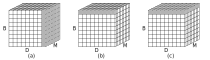
\includegraphics[width=0.7\linewidth]{kws/images/normcubes}
	\caption{Each cube represents a batch of data where $B$ is the instances axis (with the batch size), $M$ is the channels axis and $D$ is the spatial/temporal dimension. (a) represents \textit{batch normalization}, (b) is \textit{instance normalization} and (c) shows \textit{layer normalization}. The shaded areas in the cubes represent the dimensions that are aggregated in each case for computing the statistics used to normalize the data (generally the mean and the standard deviation). As it can be noticed, the only normalization technique that depends on instances of data in the batch is the \textit{batch normalization}, that is why it is more sensitive to train-test distribution differences. As it can be noticed in the picture, \textit{instance normalization} is a specific version of \textit{layer normalization} where each channel is normalized separately}
	\label{fig:normcubes}
\end{figure}




\section{Results} \label{sec:results}
The train/development/test split provided by the authors of the data set \cite{speechcommands} has been used as \textit{cross validation} (CV) setting in order to facilitate future benchmarking efforts. A simple split CV has been used instead of K-fold CV for the following reasons: (1) these models are expensive to train. Forty deep models (2 data set versions $\times$ 4 tasks $\times$ 5 random initializations) were trained per experiment. If we added K-Fold CV it would become unfeasible; (2) for the sake of reproducibility and benchmarking, as the authors of the dataset provide a default list of clips to use as validation and test.

Versions V1 and V2 of the data set have 16,000 and 9,981 hold out samples for development purposes and 16,000 and 11,005 hold out samples for testing purposes, respectively. The development set has been used to manually tune the hyperparameters and for \textit{early stopping} purposes. The model has been trained for 50 epochs in each case, with a batch size of 32 clips, and the weights of the epoch that achieved the best performance in the development set were checkpointed. The checkpointed models have been used to calculate and report the performance of the algorithm.

 The source code that has been used for this study has been uploaded to \textit{GitHub} and can be found here: \url{https://github.com/ivallesp/Xception1d}

All the results shown in this section have been measured over the test set. Five different models have been trained for each task in order to explore and report the effect of different random initializations of the weights of the network. With the aim of providing a baseline, human performance has been measured by 4 human subjects, who manually labeled $\sim 1000$ commands achieving different results. These results are reported in Table \ref{tab:comparative} along with the results of the proposed algorithm and the results reported by \cite{Andrade2018, Zhang2017, McMahan2018, Warden2018} on the matching tasks.

Besides the global results, Figure \ref{fig:boxplot35002} shows the precision and the recall obtained for the most complex model (\textit{35-words-recognition} for data version V2). In conjunction with this figure, precision, recall and f1-score metrics have been included in the tables of the appendix 2, at the end of the article.

\begin{figure}[ht]
	\centering
	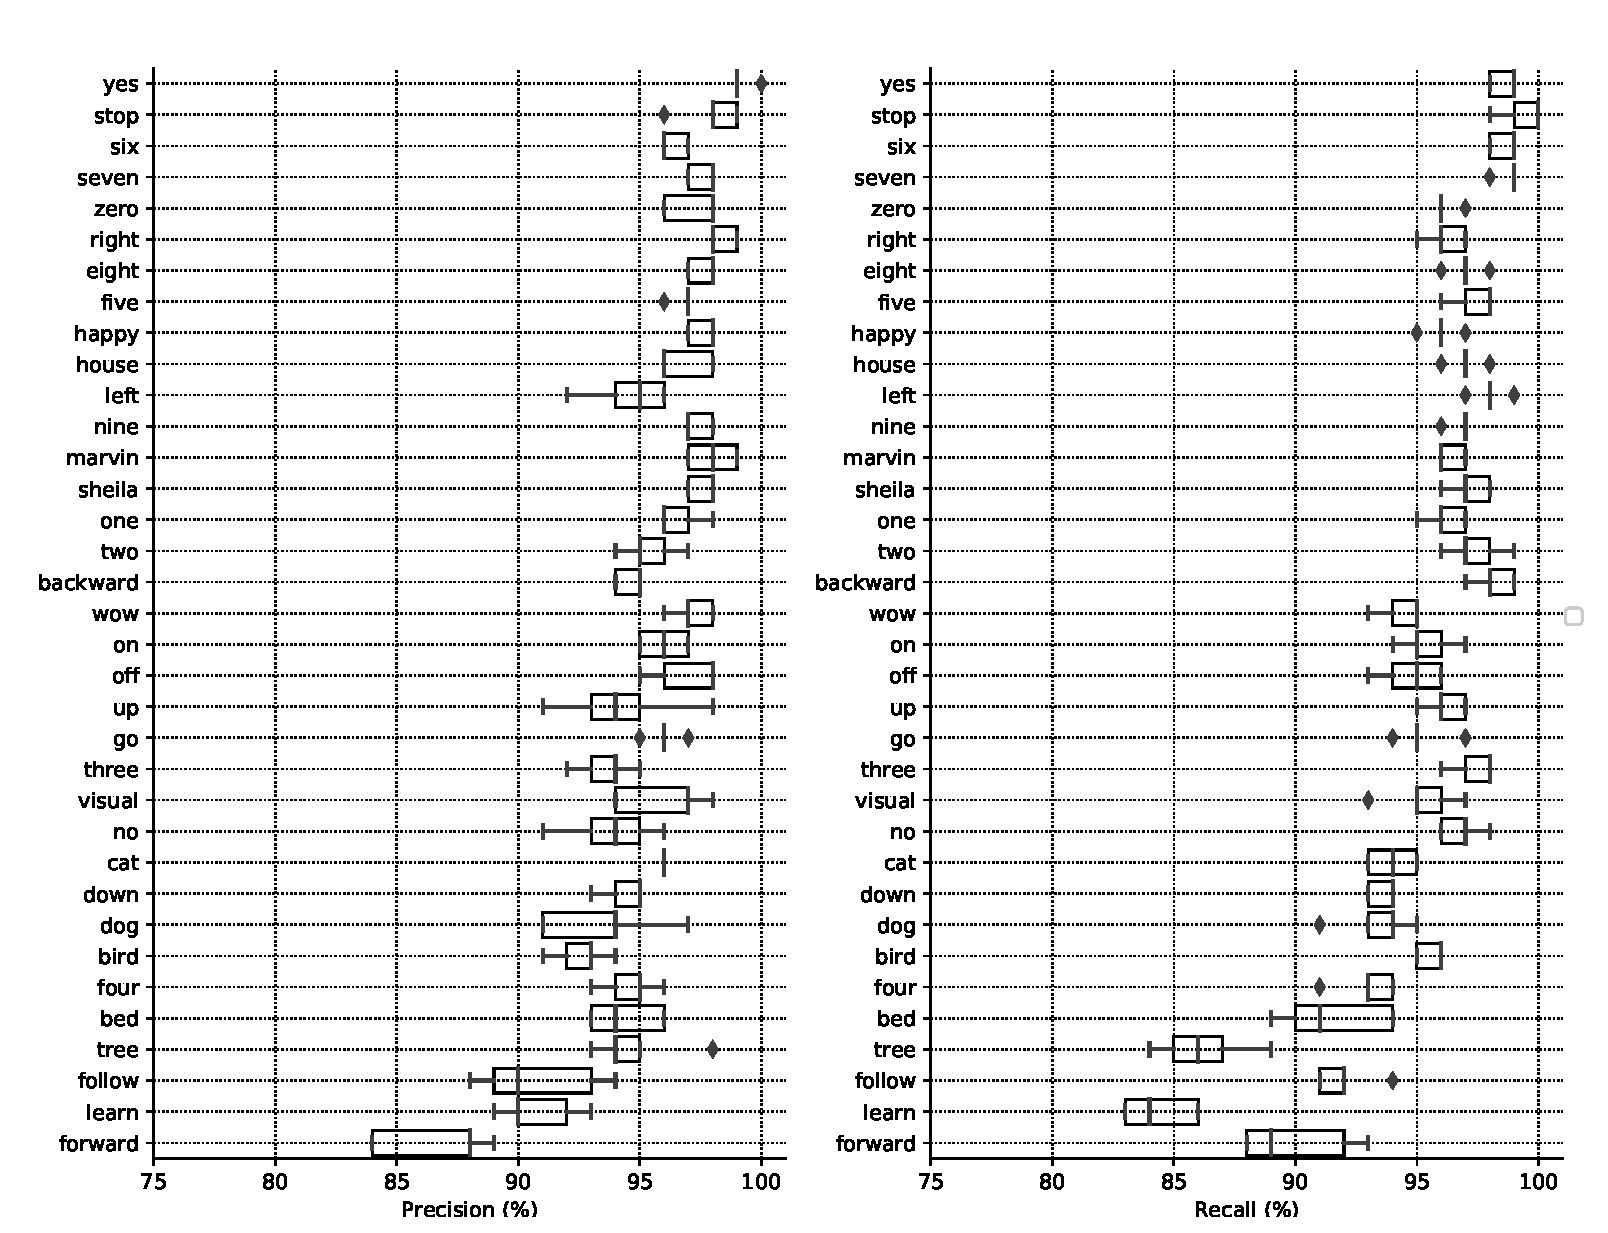
\includegraphics[width=0.8\linewidth]{kws/images/boxplot_35-words-recognition_002.eps}
	\caption{Precision and recall for each of the different classes using the \textit{35-words-recognition} model trained with data version V2. Classes are sorted by descending f1-score.}
	\label{fig:boxplot35002}
\end{figure}




\begin{table}[h!]
	\centering
	\caption{Accuracy (mean $\pm$ standard deviation) obtained by the proposed solution on the different tasks compared to other benchmark algorithms (described in \cite{Andrade2018, McMahan2018, Warden2018,Zhang2017}) and compared to our measurement of human accuracy (through 4 manual evaluations). The results of best performing algorithms for each task have been highlighted in bold in each case. Results better than human performance (given a statistical significance level of $\alpha = 0.05$) have been tagged with a star mark (*).}
	\label{tab:comparative}


	\begin{subtable}{1\textwidth}
		\caption{Results for version 1 of the data set.}
		\centering
		\scalebox{0.75}{
	\begin{tabular}{lcccccc}
		\hline
		 & Ref. \cite{Andrade2018} & Ref.  \cite{McMahan2018}\footref{foot:max} & Ref. \cite{Warden2018} & \textit{Xception-1d} & Human & p-value\footref{foot:ttest}      \\ \hline
		35-words & 94.30 & 84.35 & - & \textbf{95.85 $\pm$ 0.12 *} & 94.15 $\pm$ 1.03  & $1.46\cdot 10^{-2}$\\
		20-commands & 94.10 & 85.52 & - & \textbf{95.89 $\pm$ 0.06 *} & 94.56 $\pm$ 0.98  & $3.14\cdot 10^{-2}$\\
		10-commands & 95.60 & - & 85.40 & \textbf{97.15 $\pm$ 0.03} & 97.22 $\pm$ 0.85 & $8.75\cdot 10^{-1}$\\
		left-right & \textbf{99.20} & 95.32 & - & 98.96 $\pm$ 0.09 & 99.54 $\pm$ 0.16 & $5.24\cdot 10^{-4}$ \\ \bottomrule
	\end{tabular}}

\end{subtable}
\bigskip
\begin{subtable}{1\textwidth}
\caption{Results for version 2 of the data set.}
		\centering
\scalebox{0.75}{
\begin{tabular}{lcccccc}
	\hline
	            & Ref. \cite{Andrade2018} &   Ref. \cite{Zhang2017}\footnote{the  best results obtained among all the trials performed by the autors have been selected \label{foot:max}} & Ref. \cite{Warden2018} &           \textit{Xception-1d}           &     Human    & p-value \footnote{Student's t-test for the comparison of two means. $\alpha = 0.05$ \label{foot:ttest}} \\ \hline
	35-words    &               93.90               &               -               &            -             & \textbf{95.85 $\pm$ 0.16 *} & 94.15 $\pm$ 1.03 & $1.50\cdot 10^{-2}$ \\
	20-commands &               94.50               &               -               &            -             & \textbf{95.96 $\pm$ 0.16 *} & 94.56 $\pm$ 0.98 & $2.70\cdot 10^{-2}$\\
	10-commands &               96.90               &             95.40             &          88.20           & \textbf{97.54 $\pm$ 0.08}  & 97.22 $\pm$ 0.85 & $4.84\cdot 10^{-1}$ \\
	left-right  &          \textbf{99.40}           &               -               &            -             & 99.25 $\pm$ 0.07  & 99.54 $\pm$ 0.16 & $1.27\cdot 10^{-2}$\\ \bottomrule
\end{tabular}}
\end{subtable}
\end{table}



\section{Discussion} \label{sec:discussion}

The presented method, \textit{Xception-1d}, offers better performance than the existing methods in the literature for three out of the four tested tasks, using different sets of limited-size vocabularies. According to the results in Table \ref{tab:comparative}, \textit{Xception-1d} performed voice recognition better than the state of the art methods  \cite{Andrade2018, Zhang2017, McMahan2018, Warden2018} in three out of four tasks: \textit{35-words-recognition}, \textit{20-commands-recognition}, and \textit{10-commands-recognition}. In the only task where \textit{Xception-1d} did not achieve the best results (left-right), the leading method was the one proposed by Andrade \textit{et al}. \cite{Andrade2018} which was only marginally better ($<$0.5\% performance difference on the test set) than the presented method. \textit{Xception-1d} even surpassed human performance (with statistical significance level) in the two first tasks, including the most difficult one (\textit{35-words-recognition}).

With regard to per-class accuracy, it can be noticed from Figure \ref{fig:boxplot35002} that the algorithm performs generally well for all the classes in the most difficult scenario (35-words task) as the majority of precision and recall values lay between 90-100\%. Nonetheless, we found that the algorithm has more difficulties differentiating some groups of similar words like the following pairs: ``three'' and ``tree'', ``follow'' and ``four'', ``bed'' and ``bird'', etc. No comparison with other existing models has been included because no such detailed results have been found in the related work.

The limitation of this method is mainly linked to inherent computational cost. Depthwise separable convolutions allow for a more resource-efficient network architecture than regular convolutions, but that means that more complex architectures can be built. The tested network architectures have more than 20 million parameters, which makes training computationally expensive, even with datasets composed by a few thousands instances. Overfitting may be an issue due to this amount of parameters, but it has been prevented by using regularization with a small weight decay in all layers, and a strong dropout after the last dense layer. In spite of the aforementioned limitation, once the model has been trained with a particular vocabulary corpus, it may be locally implemented in voice-controlled systems that work in real time such as commercial speech agents.

Finally, our findings show that the per-class performance of the speech commands in the \textit{left-right} task is lower than for the other tasks (in particular the recall values). However, the per-class performance for these two classes was higher when they were included in a multiclass classification task like the \textit{35-words-recognition} task. This fact suggests that auxiliary tasks (in this case the 35-words vocabulary task) can benefit primary tasks (left-right), as more features may be extracted from more complex tasks. This hypothesis has been proven for Reinforcement Learning \cite{Jaderberg2016}, but may also apply to DL efforts.


\section{Conclusion} \label{sec:conclusion}
This work shows how a neural network architecture which succeeded in the computer vision field, with an adaption and a set of tweaks, is able to surpass human performance at a speech recognition task with limited vocabulary achieving state of the art results. This is why we suggest \textit{Xception-1d} as the \textit{de facto} architecture when facing a voice command recognition task with restricted vocabulary,  considering the computing power is not a limiting factor. The algorithm presented can have multiple  applications for improving voice-controlled systems.

A possible future line of work could be  the use of \textit{Xception-1d} architecture with a global pooling layer at the end  as an encoder of a \textit{sequence-to-sequence} architecture for tackling a speech recognition task with free vocabulary (e.g. a \textit{speech to text} engine). In addition, pruning and complexity reduction techniques may be implemented over the final network to try to reduce its computational cost.


\section*{Appendix 1}
The \textit{regular convolution} and \textit{depthwise convolution} operations \cite{howard2017}  are defined\footnote{in both cases assuming a stride of one, \textit{SAME} padding and odd size convolution kernels} in equations \ref{eq:reg_conv} and  \ref{eq:dw_conv} for illustrative purposes, where

\begin{itemize}
	\item $\mathbf{F}$ is the feature map over which the convolution operation is intended to be applied. It has a shape of $D \times M$, where $D$ represents the spatial/temporal dimension and $M$ the number of input channels.
	\item $\mathbf{K}$ is the convolution kernel and has a shape of $S \times M$ where $S$ is the size of the kernel.
	\item $\mathbf{G}$ is the output tensor produced by applying the \textit{regular convolution} operation with the filter $K$ over the input $F$ resulting in a vector of length $D$.
	\item $\hat{\mathbf{G}}$ is the output tensor produced by applying the \textit{depthwise convolution} with the filter $K$ over the input $F$, resulting in a matrix with shape $D \times M$. The number of output channels is restricted to be equal to the number of input channels $M$.
\end{itemize}


\begin{equation}
\mathbf{G}_{x} = \sum_{s, m}^{S,M} \mathbf{K}_{s, m} \cdot \mathbf{F}_{x+s-\frac{S-1}{2}, m}
\label{eq:reg_conv}
\end{equation}

\begin{equation}
\hat{\mathbf{G}}_{x, m} = \sum_{s}^{S} \mathbf{K}_{s, m} \cdot \mathbf{F}_{x+s-\frac{S-1}{2}, m}
\label{eq:dw_conv}
\end{equation}

See that $\mathbf{G}_{x} =  \sum_{m}^{M} \hat{\mathbf{G}}_{x, m}$. A \textit{pointwise convolution} would be equivalent of applying a \textit{regular} convolution with $S=1$.

The \textit{depthwise separable convolution} is composite function of a \textit{pointwise convolution} and a \textit{depthwise convolution} as follows: $PW(DW(F,W_{d}),W_{p})$ where $PW$ and $DW$ refer to the \textit{pointwise} and \textit{depthwise convolutions}, and $W_{p}$, $W_{d}$ to their weights, similarly.

The \textit{regular convolution} layer targeting $N$ output channels has a computational cost of $D \cdot M \cdot N \cdot S$. The \textit{depthwise convolution} has a computational cost of $D \cdot M \cdot S$,  and the \textit{separable convolution} $D \cdot M \cdot N$. Therefore the \textit{depthwise separable convolution} has a computational cost  of $D \cdot M  \cdot S + D \cdot M \cdot N$, i.e. the sum of its two constituting operations. Hence, by using the \textit{depthwise separable convolution} in place of the \textit{regular} one we have a cost reduction of:

$$ \frac{D \cdot M \cdot S  + D \cdot M \cdot N} {D \cdot M \cdot N \cdot S} = \frac{1}{N} + \frac{1}{S} $$


\newpage

\section*{Appendix 2}

\begin{table}[h!] \centering \scriptsize
	\caption{Detailed results for task \textit{35-words-recognition} and V1 data set, in decreasing f1-score order. The columns ``precision'', ``recall'' and ``f1-score'' have been represented as the mean $\pm$ the standard deviation in percentage scale. }
	\begin{tabular}{lcccc}
		\toprule
		{} &       precision &          recall &        f1-score & support \\
		\midrule
		happy     &  98.00$\pm$0.89 &  97.80$\pm$0.75 &  98.00$\pm$0.63 &     180 \\
		cat       &  98.20$\pm$0.40 &  97.80$\pm$0.40 &  98.00$\pm$0.00 &     166 \\
		house     &  97.60$\pm$1.36 &  98.60$\pm$0.49 &  97.80$\pm$0.75 &     150 \\
		dog       &  97.80$\pm$0.75 &  98.00$\pm$0.00 &  97.80$\pm$0.40 &     180 \\
		marvin    &  99.00$\pm$0.63 &  96.80$\pm$0.75 &  97.80$\pm$0.40 &     162 \\
		stop      &  97.20$\pm$1.47 &  98.20$\pm$0.40 &  97.60$\pm$1.02 &     249 \\
		yes       &  98.60$\pm$1.02 &  96.40$\pm$0.80 &  97.40$\pm$0.49 &     256 \\
		sheila    &  97.20$\pm$1.33 &  97.00$\pm$0.63 &  97.20$\pm$0.75 &     186 \\
		wow       &  96.80$\pm$1.17 &  97.40$\pm$0.49 &  97.20$\pm$0.40 &     165 \\
		seven     &  95.80$\pm$1.47 &  98.40$\pm$0.80 &  97.20$\pm$0.40 &     239 \\
		four      &  96.40$\pm$0.80 &  97.20$\pm$0.75 &  97.00$\pm$0.63 &     253 \\
		two       &  95.80$\pm$1.33 &  97.60$\pm$0.49 &  96.80$\pm$0.75 &     264 \\
		nine      &  95.40$\pm$1.50 &  98.20$\pm$0.75 &  96.80$\pm$0.40 &     259 \\
		on        &  95.80$\pm$1.60 &  97.00$\pm$0.63 &  96.60$\pm$1.02 &     246 \\
		six       &  95.80$\pm$0.40 &  97.20$\pm$0.40 &  96.40$\pm$0.49 &     244 \\
		bird      &  95.80$\pm$0.98 &  96.40$\pm$0.49 &  96.20$\pm$0.75 &     158 \\
		eight     &  96.80$\pm$1.94 &  95.40$\pm$0.49 &  96.00$\pm$0.89 &     257 \\
		five      &  96.00$\pm$0.63 &  96.00$\pm$0.63 &  96.00$\pm$0.63 &     271 \\
		one       &  98.00$\pm$0.89 &  93.80$\pm$1.33 &  95.80$\pm$0.40 &     248 \\
		down      &  96.00$\pm$0.63 &  95.00$\pm$0.89 &  95.60$\pm$0.80 &     253 \\
		bed       &  95.00$\pm$1.67 &  96.20$\pm$1.47 &  95.40$\pm$1.02 &     176 \\
		left      &  93.00$\pm$1.67 &  97.20$\pm$0.40 &  95.20$\pm$0.75 &     267 \\
		off       &  96.80$\pm$1.47 &  94.00$\pm$1.26 &  95.20$\pm$0.40 &     262 \\
		right     &  97.40$\pm$1.20 &  92.80$\pm$0.40 &  95.20$\pm$0.40 &     259 \\
		zero      &  95.60$\pm$1.36 &  94.40$\pm$1.02 &  95.00$\pm$0.63 &     250 \\
		up        &  94.80$\pm$0.75 &  94.80$\pm$0.98 &  94.80$\pm$0.75 &     272 \\
		no        &  94.60$\pm$1.02 &  93.00$\pm$0.89 &  93.80$\pm$1.17 &     252 \\
		go        &  94.60$\pm$1.62 &  93.40$\pm$0.80 &  93.80$\pm$0.75 &     251 \\
		tree      &  92.40$\pm$1.50 &  90.60$\pm$1.36 &  91.60$\pm$0.49 &     193 \\
		three     &  89.60$\pm$0.49 &  92.80$\pm$0.75 &  91.20$\pm$0.40 &     267 \\
		\midrule avg/total &  96.00$\pm$0.00 &  96.00$\pm$0.00 &  96.00$\pm$0.00 &    6835 \\
		\bottomrule
	\end{tabular}

\end{table}


\begin{table}[h!] \centering \scriptsize
	\caption{Detailed results for task \textit{35-words-recognition} and V2 data set, in decreasing f1-score order. The columns ``precision'', ``recall'' and ``f1-score'' have been represented as the mean $\pm$ the standard deviation in percentage scale. }
	\begin{tabular}{lcccc}
		\toprule
		{} &       precision &          recall &        f1-score & support \\
		\midrule
		yes       &  99.20$\pm$0.40 &  98.60$\pm$0.49 &  99.00$\pm$0.00 &     419 \\
		stop      &  98.00$\pm$1.10 &  99.40$\pm$0.80 &  98.60$\pm$0.49 &     411 \\
		seven     &  97.60$\pm$0.49 &  98.80$\pm$0.40 &  98.40$\pm$0.49 &     406 \\
		six       &  96.40$\pm$0.49 &  98.60$\pm$0.49 &  97.60$\pm$0.49 &     394 \\
		right     &  98.40$\pm$0.49 &  96.20$\pm$0.75 &  97.40$\pm$0.49 &     396 \\
		sheila    &  97.60$\pm$0.49 &  97.20$\pm$0.75 &  97.20$\pm$0.75 &     212 \\
		nine      &  97.40$\pm$0.49 &  96.80$\pm$0.40 &  97.20$\pm$0.40 &     408 \\
		eight     &  97.60$\pm$0.49 &  97.00$\pm$0.63 &  97.20$\pm$0.40 &     408 \\
		marvin    &  98.00$\pm$0.89 &  96.40$\pm$0.49 &  97.20$\pm$0.40 &     195 \\
		five      &  96.80$\pm$0.40 &  97.40$\pm$0.80 &  97.00$\pm$0.00 &     445 \\
		house     &  96.80$\pm$0.98 &  97.00$\pm$0.63 &  96.80$\pm$0.75 &     191 \\
		happy     &  97.60$\pm$0.49 &  96.00$\pm$0.63 &  96.80$\pm$0.40 &     203 \\
		zero      &  97.20$\pm$0.98 &  96.20$\pm$0.40 &  96.60$\pm$0.49 &     418 \\
		left      &  94.60$\pm$1.50 &  98.00$\pm$0.63 &  96.40$\pm$0.80 &     412 \\
		backward  &  94.60$\pm$0.49 &  98.20$\pm$0.75 &  96.40$\pm$0.49 &     165 \\
		one       &  96.60$\pm$0.80 &  96.20$\pm$0.75 &  96.40$\pm$0.49 &     399 \\
		two       &  95.40$\pm$1.02 &  97.40$\pm$1.02 &  96.20$\pm$0.75 &     424 \\
		wow       &  97.20$\pm$0.75 &  94.40$\pm$0.80 &  96.00$\pm$0.89 &     206 \\
		off       &  97.00$\pm$1.26 &  94.80$\pm$1.17 &  95.80$\pm$0.75 &     402 \\
		on        &  96.00$\pm$0.89 &  95.40$\pm$1.02 &  95.80$\pm$0.40 &     396 \\
		visual    &  96.00$\pm$1.67 &  95.20$\pm$1.33 &  95.60$\pm$0.80 &     165 \\
		go        &  96.00$\pm$0.63 &  95.20$\pm$0.98 &  95.40$\pm$0.49 &     402 \\
		no        &  93.80$\pm$1.72 &  96.80$\pm$0.75 &  95.40$\pm$0.49 &     405 \\
		up        &  94.20$\pm$2.32 &  96.20$\pm$0.75 &  95.20$\pm$0.98 &     425 \\
		cat       &  96.00$\pm$0.00 &  94.00$\pm$0.89 &  95.20$\pm$0.75 &     194 \\
		three     &  93.60$\pm$1.02 &  97.40$\pm$0.80 &  95.20$\pm$0.75 &     405 \\
		four      &  94.60$\pm$1.02 &  93.00$\pm$1.10 &  94.00$\pm$0.63 &     400 \\
		bird      &  92.60$\pm$1.02 &  95.60$\pm$0.49 &  94.00$\pm$0.63 &     185 \\
		down      &  94.40$\pm$0.80 &  93.60$\pm$0.49 &  94.00$\pm$0.00 &     406 \\
		dog       &  93.40$\pm$2.24 &  93.40$\pm$1.36 &  93.40$\pm$0.80 &     220 \\
		bed       &  94.40$\pm$1.36 &  91.60$\pm$2.06 &  93.20$\pm$1.17 &     207 \\
		follow    &  90.80$\pm$2.32 &  92.00$\pm$1.10 &  91.60$\pm$1.36 &     172 \\
		tree      &  94.80$\pm$1.72 &  86.20$\pm$1.72 &  90.40$\pm$1.20 &     193 \\
		forward   &  86.60$\pm$2.15 &  90.00$\pm$2.10 &  88.20$\pm$1.72 &     155 \\
		learn     &  90.80$\pm$1.47 &  84.40$\pm$1.36 &  87.60$\pm$1.02 &     161 \\
		\midrule avg/total &  96.00$\pm$0.00 &  96.00$\pm$0.00 &  96.00$\pm$0.00 &   11005 \\
		\bottomrule
	\end{tabular}

\end{table}



\begin{table} \centering \scriptsize
	\caption{Detailed results for task \textit{20-commands-recognition} V1 data set, in decreasing f1-score order. The columns ``precision'', ``recall'' and ``f1-score'' have been represented as the mean $\pm$ the standard deviation in percentage scale. }
	\begin{tabular}{lcccc}
		\toprule
		{} &       precision &          recall &        f1-score & support \\
		\midrule
		nine      &  97.80$\pm$1.17 &  97.60$\pm$1.02 &  97.80$\pm$0.40 &     259 \\
		stop      &  97.00$\pm$1.79 &  98.00$\pm$0.63 &  97.60$\pm$1.02 &     249 \\
		yes       &  98.60$\pm$0.80 &  96.40$\pm$0.49 &  97.60$\pm$0.49 &     256 \\
		seven     &  96.40$\pm$0.49 &  98.20$\pm$0.75 &  97.40$\pm$0.49 &     239 \\
		six       &  97.20$\pm$0.75 &  97.40$\pm$0.49 &  97.20$\pm$0.40 &     244 \\
		unknown   &  96.60$\pm$0.49 &  97.00$\pm$0.00 &  97.00$\pm$0.00 &    1716 \\
		on        &  96.40$\pm$1.20 &  97.20$\pm$0.40 &  96.80$\pm$0.40 &     246 \\
		five      &  96.80$\pm$1.17 &  95.60$\pm$0.80 &  96.20$\pm$0.75 &     271 \\
		one       &  98.00$\pm$0.63 &  94.20$\pm$0.40 &  96.20$\pm$0.40 &     248 \\
		zero      &  96.60$\pm$1.50 &  94.60$\pm$1.02 &  95.80$\pm$0.98 &     250 \\
		four      &  94.00$\pm$1.10 &  97.60$\pm$0.49 &  95.80$\pm$0.75 &     253 \\
		two       &  94.80$\pm$1.60 &  96.40$\pm$0.80 &  95.60$\pm$1.02 &     264 \\
		left      &  93.60$\pm$1.02 &  97.20$\pm$0.75 &  95.40$\pm$0.80 &     267 \\
		eight     &  95.60$\pm$0.49 &  95.40$\pm$0.80 &  95.40$\pm$0.49 &     257 \\
		right     &  96.60$\pm$1.02 &  93.80$\pm$1.17 &  95.20$\pm$0.98 &     259 \\
		off       &  97.20$\pm$1.17 &  93.60$\pm$1.02 &  95.20$\pm$0.75 &     262 \\
		up        &  95.80$\pm$0.40 &  94.40$\pm$1.50 &  95.00$\pm$0.63 &     272 \\
		down      &  95.80$\pm$0.75 &  93.40$\pm$0.80 &  94.60$\pm$0.49 &     253 \\
		no        &  93.20$\pm$1.33 &  94.80$\pm$0.75 &  94.00$\pm$0.63 &     252 \\
		go        &  94.00$\pm$1.55 &  91.40$\pm$1.62 &  92.60$\pm$0.49 &     251 \\
		three     &  91.00$\pm$0.89 &  92.00$\pm$1.55 &  91.40$\pm$1.02 &     267 \\
		\midrule avg/total &  96.00$\pm$0.00 &  96.00$\pm$0.00 &  96.00$\pm$0.00 &    6835 \\
		\bottomrule
	\end{tabular}

\end{table}



\begin{table} \centering \scriptsize
	\caption{Detailed results for task \textit{20-commands-recognition} and data version V2, sorted by decreasing f1-score order. The columns ``precision'', ``recall'' and ``f1-score'' have been represented as the mean $\pm$ the standard deviation in percentage scale. }
	\begin{tabular}{lcccc}
		\toprule
		{} &       precision &          recall &        f1-score & support \\
		\midrule
		seven     &  98.80$\pm$0.40 &  98.60$\pm$0.49 &  98.80$\pm$0.40 &     406 \\
		yes       &  98.80$\pm$0.40 &  98.60$\pm$0.49 &  98.60$\pm$0.49 &     419 \\
		stop      &  98.80$\pm$0.40 &  99.00$\pm$0.63 &  98.60$\pm$0.49 &     411 \\
		six       &  97.60$\pm$1.02 &  98.20$\pm$0.75 &  97.60$\pm$0.49 &     394 \\
		eight     &  98.00$\pm$0.63 &  96.40$\pm$0.49 &  97.00$\pm$0.00 &     408 \\
		zero      &  97.80$\pm$0.75 &  96.40$\pm$0.49 &  96.80$\pm$0.40 &     418 \\
		nine      &  98.00$\pm$0.63 &  95.40$\pm$0.49 &  96.60$\pm$0.49 &     408 \\
		right     &  97.40$\pm$1.36 &  96.00$\pm$0.89 &  96.60$\pm$0.49 &     396 \\
		two       &  95.80$\pm$0.75 &  96.80$\pm$0.75 &  96.40$\pm$0.49 &     424 \\
		five      &  96.60$\pm$1.02 &  95.40$\pm$1.20 &  96.00$\pm$0.63 &     445 \\
		one       &  97.40$\pm$0.49 &  95.00$\pm$0.00 &  96.00$\pm$0.00 &     399 \\
		left      &  94.40$\pm$0.80 &  97.60$\pm$0.49 &  96.00$\pm$0.00 &     412 \\
		off       &  97.20$\pm$0.75 &  94.60$\pm$1.20 &  95.80$\pm$0.75 &     402 \\
		no        &  95.20$\pm$1.47 &  96.40$\pm$0.49 &  95.80$\pm$0.75 &     405 \\
		on        &  95.60$\pm$1.62 &  95.20$\pm$0.75 &  95.40$\pm$0.49 &     396 \\
		up        &  95.40$\pm$0.49 &  95.20$\pm$0.40 &  95.40$\pm$0.49 &     425 \\
		three     &  94.40$\pm$1.02 &  96.20$\pm$1.17 &  95.00$\pm$0.00 &     405 \\
		unknown   &  94.40$\pm$0.49 &  96.00$\pm$0.63 &  95.00$\pm$0.00 &    2824 \\
		go        &  95.00$\pm$1.41 &  94.80$\pm$0.75 &  94.80$\pm$0.40 &     402 \\
		down      &  94.80$\pm$0.40 &  93.40$\pm$0.49 &  94.20$\pm$0.40 &     406 \\
		four      &  95.20$\pm$0.98 &  92.00$\pm$1.67 &  93.60$\pm$0.49 &     400 \\
		\midrule avg/total &  96.00$\pm$0.00 &  96.00$\pm$0.00 &  96.00$\pm$0.00 &   11005 \\
		\bottomrule
	\end{tabular}

\end{table}



\begin{table} \centering \scriptsize
	\caption{Detailed results for task \textit{10-commands-recognition} and data version V1, sorted by decreasing f1-score order. The columns ``precision'', ``recall'' and ``f1-score'' have been represented as the mean $\pm$ the standard deviation in percentage scale. }
	\begin{tabular}{lcccc}
		\toprule
		{} &       precision &          recall &        f1-score & support \\
		\midrule
		unknown   &  97.60$\pm$0.49 &  99.00$\pm$0.00 &  98.20$\pm$0.40 &    4268 \\
		stop      &  98.20$\pm$1.17 &  97.60$\pm$0.80 &  97.80$\pm$0.40 &     249 \\
		yes       &  98.60$\pm$1.50 &  95.60$\pm$0.80 &  97.00$\pm$0.89 &     256 \\
		on        &  97.60$\pm$1.02 &  95.80$\pm$0.40 &  96.80$\pm$0.40 &     246 \\
		left      &  95.60$\pm$1.02 &  95.60$\pm$0.80 &  95.60$\pm$0.49 &     267 \\
		right     &  96.60$\pm$1.50 &  92.80$\pm$0.75 &  94.40$\pm$0.80 &     259 \\
		up        &  95.60$\pm$1.36 &  93.00$\pm$0.89 &  94.40$\pm$0.80 &     272 \\
		off       &  96.40$\pm$1.50 &  92.40$\pm$1.50 &  94.40$\pm$0.49 &     262 \\
		down      &  95.40$\pm$0.49 &  92.80$\pm$0.75 &  94.20$\pm$0.40 &     253 \\
		no        &  94.80$\pm$0.75 &  91.80$\pm$0.40 &  93.20$\pm$0.40 &     252 \\
		go        &  93.60$\pm$2.24 &  92.40$\pm$1.62 &  92.80$\pm$1.33 &     251 \\
		\midrule avg/total &  97.00$\pm$0.00 &  97.00$\pm$0.00 &  97.00$\pm$0.00 &    6835 \\
		\bottomrule
	\end{tabular}

\end{table}



\begin{table} \centering \scriptsize
	\caption{Detailed results for task \textit{10-commands-recognition} and data version V2, sorted by decreasing f1-score order. The columns ``precision'', ``recall'' and ``f1-score'' have been represented as the mean $\pm$ the standard deviation in percentage scale. }
	\begin{tabular}{lcccc}
		\toprule
		{} &       precision &          recall &        f1-score & support \\
		\midrule
		unknown   &  98.20$\pm$0.40 &  99.00$\pm$0.00 &  99.00$\pm$0.00 &    6931 \\
		yes       &  99.00$\pm$0.63 &  98.40$\pm$0.49 &  98.80$\pm$0.40 &     419 \\
		stop      &  98.40$\pm$0.49 &  98.60$\pm$0.49 &  98.40$\pm$0.49 &     411 \\
		right     &  97.80$\pm$0.75 &  95.60$\pm$1.02 &  96.80$\pm$0.75 &     396 \\
		left      &  94.40$\pm$1.02 &  97.40$\pm$0.49 &  95.80$\pm$0.40 &     412 \\
		go        &  95.40$\pm$1.02 &  94.80$\pm$0.75 &  95.00$\pm$0.63 &     402 \\
		up        &  96.20$\pm$0.75 &  93.60$\pm$0.49 &  95.00$\pm$0.00 &     425 \\
		no        &  93.80$\pm$1.33 &  95.20$\pm$1.33 &  94.80$\pm$0.75 &     405 \\
		off       &  95.40$\pm$0.80 &  93.80$\pm$0.40 &  94.60$\pm$0.49 &     402 \\
		on        &  95.60$\pm$1.02 &  93.80$\pm$0.75 &  94.40$\pm$0.49 &     396 \\
		down      &  94.80$\pm$0.98 &  93.00$\pm$0.89 &  94.00$\pm$0.63 &     406 \\
		\midrule avg/total &  97.60$\pm$0.49 &  97.60$\pm$0.49 &  97.60$\pm$0.49 &   11005 \\
		\bottomrule
	\end{tabular}

\end{table}



\begin{table} \centering \scriptsize
	\caption{Detailed results for task \textit{left-right} and data version V1, sorted by decreasing f1-score order. The columns ``precision'', ``recall'' and ``f1-score'' have been represented as the mean $\pm$ the standard deviation in percentage scale. }
	\begin{tabular}{lcccc}
		\toprule
		{} &       precision &           recall &        f1-score & support \\
		\midrule
		unknown   &  99.00$\pm$0.00 &  100.00$\pm$0.00 &  99.20$\pm$0.40 &    6309 \\
		left      &  95.40$\pm$1.96 &   92.00$\pm$0.89 &  93.60$\pm$0.80 &     267 \\
		right     &  96.20$\pm$1.94 &   87.60$\pm$1.85 &  91.80$\pm$0.75 &     259 \\
		\midrule avg/total &  99.00$\pm$0.00 &   99.00$\pm$0.00 &  99.00$\pm$0.00 &    6835 \\
		\bottomrule
	\end{tabular}

\end{table}



\begin{table} \centering \scriptsize
	\caption{Detailed results for task \textit{left-right} and data version V2, sorted by decreasing f1-score order. The columns ``precision'', ``recall'' and ``f1-score'' have been represented as the mean $\pm$ the standard deviation in percentage scale. }
	\begin{tabular}{lcccc}
		\toprule
		{} &       precision &           recall &         f1-score & support \\
		\midrule
		left      &  95.80$\pm$0.98 &   94.00$\pm$0.89 &   95.00$\pm$0.63 &     412 \\
		right     &  98.20$\pm$1.47 &   90.60$\pm$2.65 &   94.00$\pm$1.10 &     396 \\
		unknown   &  99.40$\pm$0.49 &  100.00$\pm$0.00 &  100.00$\pm$0.00 &   10197 \\
		\midrule avg/total &  99.00$\pm$0.00 &   99.00$\pm$0.00 &   99.00$\pm$0.00 &   11005 \\
		\bottomrule
	\end{tabular}

\end{table}

